\subsubsection{Sectors Operations}
\label{sec:geo_sectors_ops}  

How to define sectors attributes is defined in \nameref{sec:ui_configure_sectors}. \\

For each defined sector, a colored polygon is shown, grouped by its layer. Such a structure could look as follows:

\begin{itemize}
 \item Layer A
 \begin{itemize}
 \item Sector A1
 \item Sector A2
\end{itemize} 
 \item Layer B
  \begin{itemize}
 \item Sector B1
\end{itemize} 
\end{itemize}

Each layer or sector can be shown/hidden. The sectors layer display configuration is stored in the configuration and restored upon startup. \\

For the examples shown in the respective task, the following display can be shown:

\begin{figure}[H]
    \centering
    \hspace*{-2.5cm}
    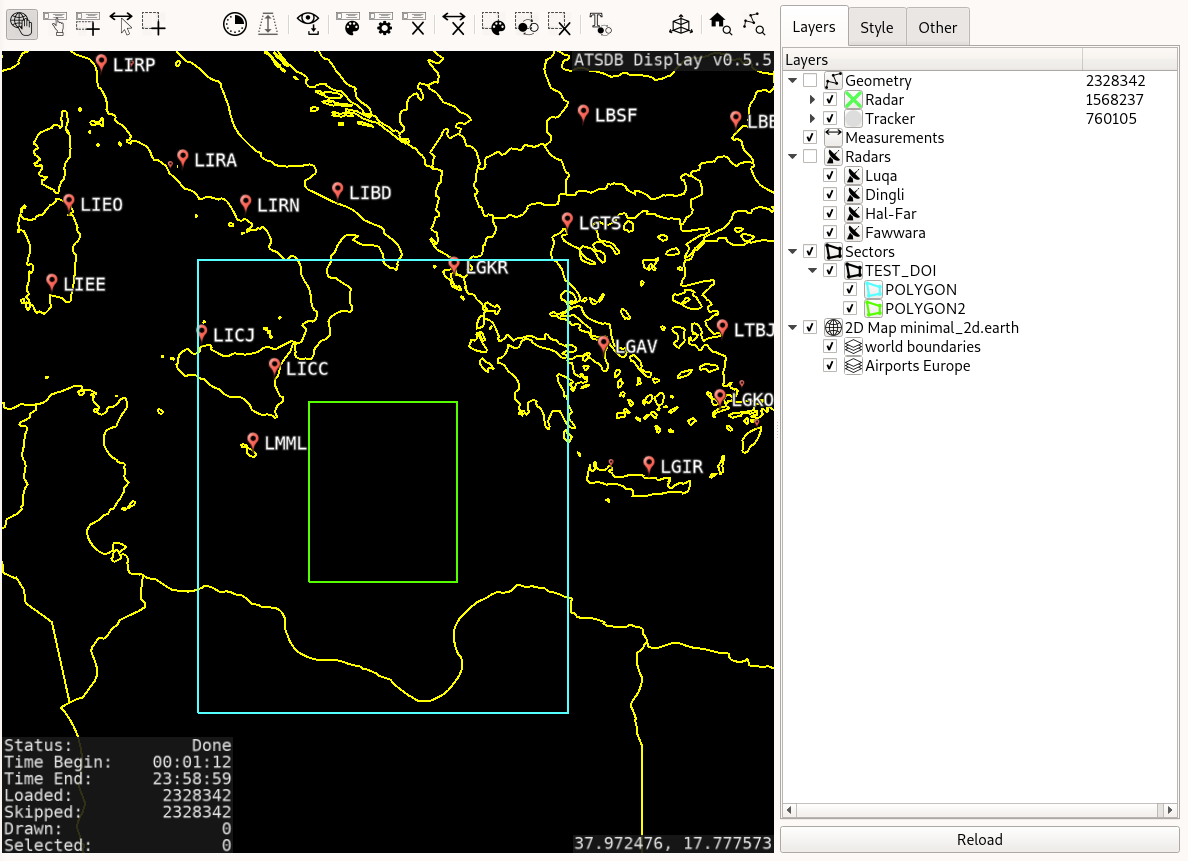
\includegraphics[width=19cm]{figures/geoview_sectors2d.png}
  \caption{Geographic View with 2D Sector Examples}
\end{figure}

\begin{figure}[H]
    \centering
    \hspace*{-2.5cm}
    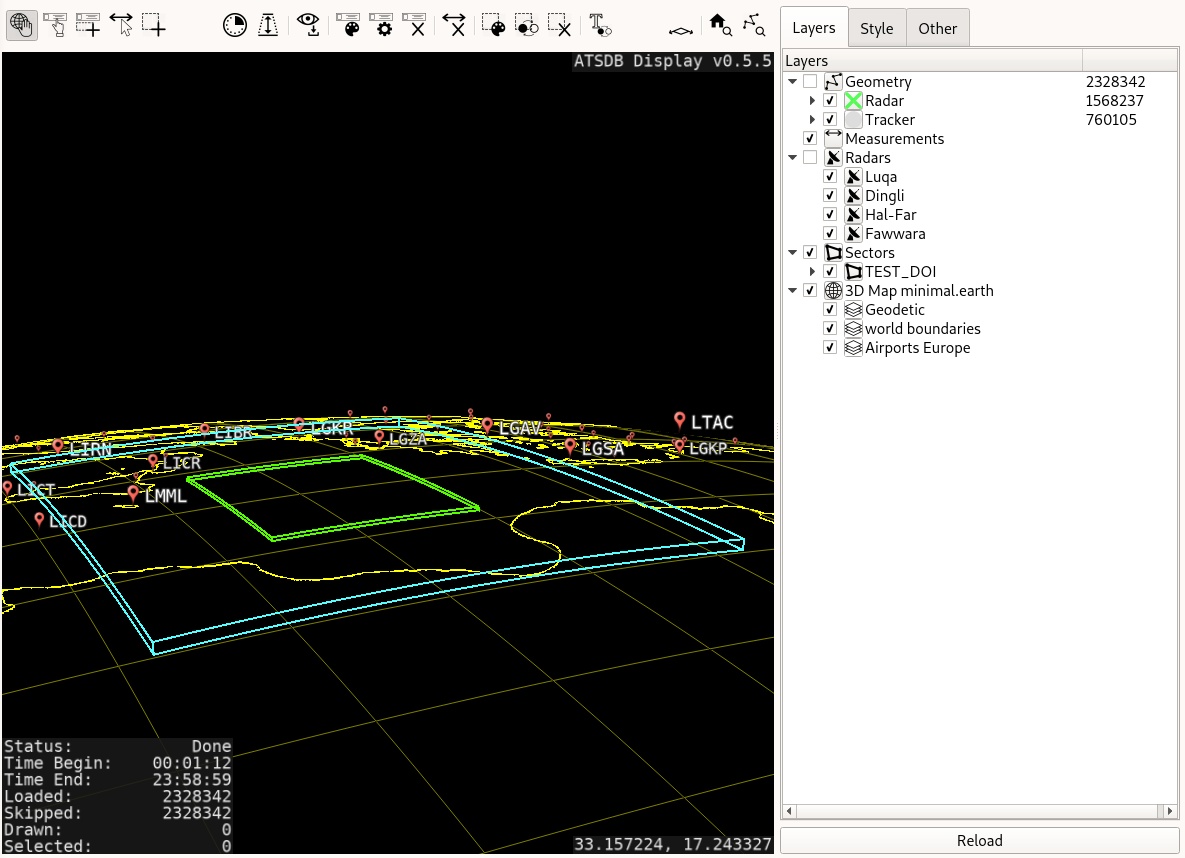
\includegraphics[width=19cm]{figures/geoview_sectors3d.png}
  \caption{Geographic View with 3D Sector Examples}
\end{figure}

\paragraph{Sector Editing}
\label{sec:geo_sectors_editing}

Sectors of the active Data Context can be created, drawn, edited, renamed, colored and deleted in the Geographic View. Use a right-click on a tree item in the Layers widget to open its context menu. \\

\begin{itemize}
 \item Each change is saved into the active Data Context at once, and into the database if one is open
 \item Each change updates the sectors in all Views, the sectors filter, the Reconstructor and the Evaluation
 \item The exclusion flag and the altitude limits of a sector are not edited here. Use \nameref{sec:ui_configure_sectors} for these
\end{itemize}
\ \\


\includegraphics[width=0.5cm]{../../data/icons/hint.png} \textbf{Please note that all sector edit actions are disabled in Live Mode: Running and while a sector edit is active. The tooltip of a disabled action shows the reason.} \\

\begin{figure}[H]
  \center
    \fbox{\parbox{0.8\textwidth}{\vspace{1.5cm}\centering \textcolor{red}{\textbf{[FIGURE TODO: Layers widget, context menu of a sector layer open with Add New..., Rename Layer..., Set Color..., Delete All]}}\vspace{1.5cm}}}
  \caption{Geographic View Sector Layer Context Menu}
\end{figure}

The context menu actions are as follows:

\begin{center}
 \begin{tabularx}{\textwidth}{ | l | l | X |}
  \hline
  \textbf{Item} & \textbf{Action} & \textbf{Description} \\
  \hline
  \hline
  Sectors & Add New... & Draw a new sector, then enter the layer name, the sector name and the color \\
  \hline
  Sectors & Delete All & Delete all sectors of the active Data Context, after confirmation \\
  \hline
  Sector Layer & Add New... & Draw a new sector in this layer, then enter the sector name \\
  \hline
  Sector Layer & Rename Layer... & Rename the sector layer \\
  \hline
  Sector Layer & Set Color... & Set the color of all sectors in the layer \\
  \hline
  Sector Layer & Delete All & Delete the sector layer with all its sectors, after confirmation \\
  \hline
  Sector & Edit Polygon & Move, add and delete the vertices of the sector on the map \\
  \hline
  Sector & Rename... & Rename the sector \\
  \hline
  Sector & Set Color... & Set the color of the sector \\
  \hline
  Sector & Delete & Delete the sector, after confirmation \\
  \hline
 \end{tabularx}
\end{center}
\ \\

Names:
\begin{itemize}
 \item A layer name must be unique in the Data Context
 \item A sector name must be unique in its layer
 \item An empty or existing name is refused, the dialog stays open and shows the reason
\end{itemize}
\ \\

The New Sector Layer dialog is shown after a new sector is drawn with Add New... on the Sectors item. It contains:
\begin{itemize}
 \item Layer Name: name of the new sector layer
 \item Sector Name: name of the new sector
 \item Color: color of the sectors in the layer, click to select
 \item Create: creates the layer with the sector. Disabled if a name is empty or the layer exists, the reason is shown above the button
\end{itemize}
\ \\

Colors:
\begin{itemize}
 \item A new sector in an existing layer gets the color of the other sectors in its layer
 \item The first sector of a new layer gets the color from the New Sector Layer dialog
\end{itemize}
\ \\


\includegraphics[width=0.5cm]{../../data/icons/hint.png} \textbf{Please note that a renamed sector layer is shown, also if the layer was hidden before the rename.} \\

\subparagraph{Sector Edit Tool}

Drawing and editing of a sector polygon is done with the \textbf{sector edit tool} on the map. The tool works in the same way as the polygon tools of QGIS. \\

\begin{itemize}
 \item The tool starts from the context menu only. It has no toolbar button and no keyboard shortcut
 \item While the tool is active:
 \begin{itemize}
  \item The other tools of the toolbar are disabled
  \item Mouse clicks on the map go to the tool. Selection and label toggles are not available
  \item Map navigation with the middle mouse button and the mouse wheel is possible
  \item A text in the map shows the sector name, the number of vertices and the key help
 \end{itemize}
 \item The edit is canceled if the active Data Context changes, if the sectors are changed from another place, or if a data load starts
 \item A sector must have at least 3 vertices
\end{itemize}
\ \\

\begin{figure}[H]
  \center
    \fbox{\parbox{0.8\textwidth}{\vspace{1.5cm}\centering \textcolor{red}{\textbf{[FIGURE TODO: Geographic View, sector edit tool in Edit Polygon mode, vertices and segment center nodes shown, help text visible]}}\vspace{1.5cm}}}
  \caption{Geographic View Sector Edit Tool}
\end{figure}

\textbf{Draw a New Sector} \\

Use Add New... on the Sectors item or on a sector layer. The new polygon is drawn in yellow.

\begin{center}
 \begin{tabularx}{\textwidth}{ | l | X |}
  \hline
  \textbf{Input} & \textbf{Action} \\
  \hline
  \hline
  Left click & Add a vertex \\
  \hline
  Mouse move & The polygon follows the mouse cursor \\
  \hline
  Backspace or Delete & Remove the last vertex \\
  \hline
  Right click & Finish the polygon and save the sector \\
  \hline
  Escape & Cancel, no sector is created \\
  \hline
 \end{tabularx}
\end{center}
\ \\

\begin{itemize}
 \item A finish with less than 3 vertices is a cancel
 \item After the finish, a name dialog is shown:
 \begin{itemize}
  \item Add New... on the Sectors item: the New Sector Layer dialog
  \item Add New... on a sector layer: the sector name dialog
 \end{itemize}
 \item A cancel in the name dialog goes back to the tool, the polygon stays. Escape then discards the polygon
\end{itemize}
\ \\

\textbf{Edit a Sector Polygon} \\

Use Edit Polygon on a sector. The original sector line is hidden during the edit. The vertices and the segment center nodes are shown.

\begin{center}
 \begin{tabularx}{\textwidth}{ | l | X |}
  \hline
  \textbf{Input} & \textbf{Action} \\
  \hline
  \hline
  Left click on a vertex & Start to move the vertex, the next left click places it \\
  \hline
  Left press on a vertex and drag & Move the vertex, the release places it \\
  \hline
  Left click on a segment center node & Add a vertex, it follows the mouse cursor, the next left click places it \\
  \hline
  Left click on a segment & Move the segment, the next left click places it \\
  \hline
  Double click on a segment & Add a vertex at that position, it follows the mouse cursor, the next left click places it \\
  \hline
  Shift + double click on a segment & Add a vertex at that position \\
  \hline
  Left press on the map and drag & Select the vertices in the rectangle \\
  \hline
  Shift + left click on a vertex & Add the vertex to the selection \\
  \hline
  Ctrl + left click on a vertex & Remove the vertex from the selection \\
  \hline
  Left click on a selected vertex & Move all selected vertices, the next left click places them \\
  \hline
  Delete or Backspace & Delete the selected vertices, or the vertex being moved \\
  \hline
  Escape & Cancel the current move or new vertex. With nothing in progress: cancel the edit and restore the original polygon \\
  \hline
  Right click & Cancel the current move. With nothing in progress: save the polygon and end the tool \\
  \hline
 \end{tabularx}
\end{center}
\ \\

\begin{itemize}
 \item A mouse position within 8 pixels of a vertex or a segment is a hit
 \item A drag of less than 10 pixels is a click
 \item A delete that leaves less than 3 vertices is refused
\end{itemize}
